\documentclass[11pt]{article}

% Basic setup
\usepackage{cmap}
\usepackage[utf8]{inputenc}
\usepackage[T2A]{fontenc}
\usepackage[english]{babel}

% Sans serif font by default
\renewcommand\familydefault{\sfdefault}

% Document margins
\usepackage[margin=2.5cm]{geometry}

% \includegraphics, used to include a picture of me
\usepackage{graphicx}

% === Typography ===

% == Boxes ==
\usepackage{adjustbox}
\usepackage{calc}
\usepackage{tabularx}

% == Colors ==
\usepackage[usenames,dvipsnames]{color}
\definecolor{CvRuleColor}{gray}{0.5}
\definecolor{CvWorkplaceHeaderColor}{gray}{0.97}

% == URLs ==
\usepackage[colorlinks=true,urlcolor=blue]{hyperref}

% == Paragraphs ==
\usepackage{parskip}
\setlength\parindent{0cm}
\setlength\parskip{0cm}

% == Lists ==
\usepackage{enumitem} % [noitemsep]

% === Custom commands ===

% "C++", thanks to this guy: http://tex.stackexchange.com/a/4304/9088
\usepackage{relsize}
\newcommand\CXX{C\nolinebreak[4]\hspace{-.05em}\raisebox{.4ex}{\relsize{-3}{\textbf{++}}}}

% Whitespace
\newcommand\CvSmallSkipLength{0.5em}
\newcommand\CvBigSkipLength{1em}

\newcommand\CvSkip[1]{\vspace{#1}}

\newcommand\CvSmallSkip{\CvSkip{\CvSmallSkipLength}}
\newcommand\CvBigSkip{\CvSkip{\CvBigSkipLength}}

% Section headers ("Experience", "Education", etc.)
\newcommand\CvSectionHeader[1]{\CvBigSkip\textbf{#1}\CvBigSkip}

% Horizontal line/separator
\newcommand\CvRule{\begingroup\color{CvRuleColor}\hrule\endgroup}

% Workplace header
\newcommand\CvWorkplaceHeader[5]{\begingroup%
	\CvRule%
	\fboxsep0pt%
	\colorbox{CvWorkplaceHeaderColor}{%
		\begin{minipage}{\linewidth-2\fboxsep}%
			\CvSmallSkip%
			#1 -- #2 \hfill \textit{#3} at #4 (\href{http://#5/}{#5})%
			\CvSmallSkip%
		\end{minipage}%
	}%
	\CvRule%
	\endgroup%
}

% Workplace description
\newenvironment{CvWorkplaceDescription}{%
	\begingroup\setlength\parskip{\CvSmallSkipLength}%
}{%
	\CvSmallSkip\endgroup%
}

\pagestyle{empty}

\begin{document}
	
	\adjustbox{valign=t}{%
		\begin{minipage}{3.5cm}%
			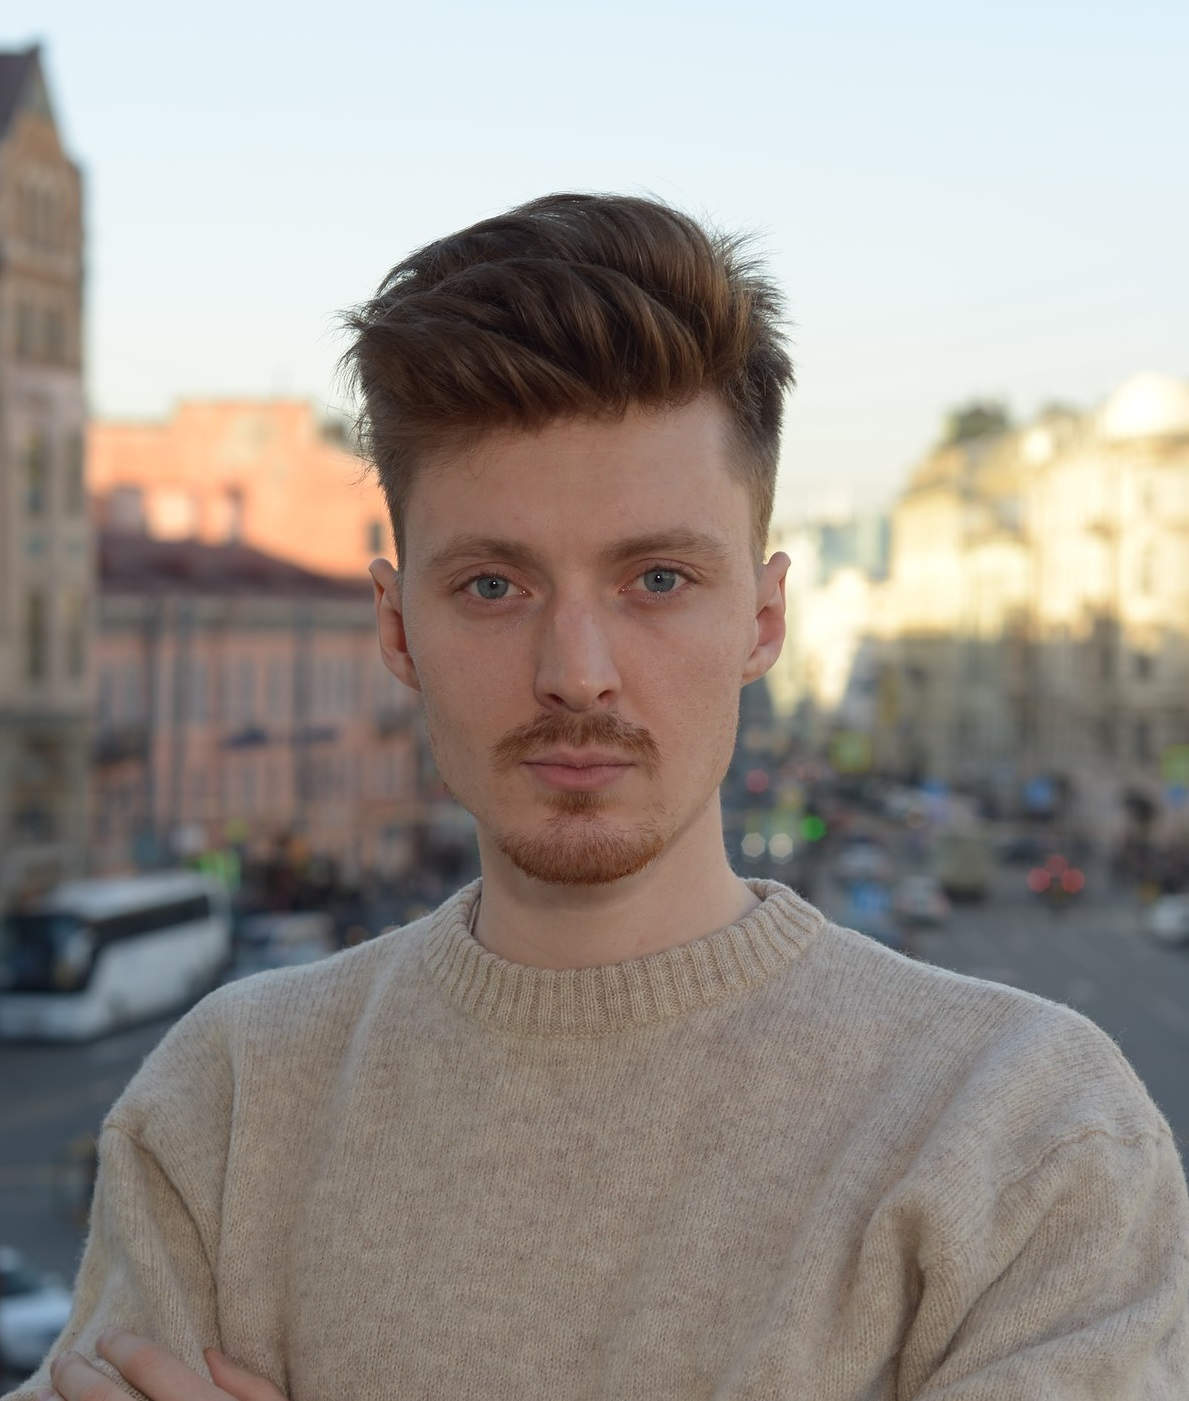
\includegraphics[width=3.5cm]{img/selfie.jpg}
		\end{minipage}%
	}%
	\hfill%
	\adjustbox{valign=t}{%
		\begin{minipage}{\linewidth-3.5cm-\CvBigSkipLength}%
			{\bfseries\large Alexey Polusov}\\*
			{Master student at IFMO Jet Brains} \\*
			{\color{CvRuleColor} Last updated on: \today}
			\CvBigSkip
			\CvRule
			\CvSmallSkip
			\begin{tabularx}{\textwidth}{@{}lX}
				email: & \href{mailto:lectricas@gmail.com}{lectricas@gmail.com} \\
				github: & \href{https://github.com/lectricas/}{https://github.com/lectricas/} \\
				tel.: & +7\,(952)\,377-09-69 \\
				Address: & 1 Kaluzhskiy Pereulok, apt. 59 \\
				& Saint Petersburg, Russia, 197198 \\
			\end{tabularx}%
			\CvSmallSkip
			\CvRule
		\end{minipage}%
	}
	
	\begin{LARGE}  
		\CvSectionHeader{Experience}
	\end{LARGE}  
	
	\CvWorkplaceHeader{February 2019}{August 2021}{Android developer}{Tinkoff}{tinkoff.ru}
	\begin{CvWorkplaceDescription}
		As my daily routine, I developed the payment section of Tinkoff mobile app. Also, I was a lecturer and a mentor in Tinkoff Fintech school.
		\begin{itemize}[noitemsep]
			\item Development.
			\begin{itemize}
				\item I make and support features like payments by phone/card, QR, shake, Bluetooth. SWIFT and CIS transfers, templates/favorites, bills and many other stuff.
				\item Payment section is the oldest and the biggest part of the Tinkoff mobile app.
				\item writing Unit and UI tests is a must in our team.
			\end{itemize}
			
			\item Fintech school.
			\begin{itemize}
				\item I participated as a lecturer and a mentor in two online schools for Android developers. 
				\item I've given a lectures on Dagger2 and networks, also reviewed Android homework. Some of my students now work in Tinkoff. 
			\end{itemize}
		\end{itemize}
		
		Key skills \& technologies employed:
		\begin{itemize}[noitemsep]
			\item Kotlin, Java, Gradle, UI tests, public speech, code review, carefulness, responsibility, time management. 
		\end{itemize}
		
		
	\end{CvWorkplaceDescription}
	
	\CvWorkplaceHeader{October 2018}{February 2019}{Lead Android developer}{Firstline Software}{firstlinesoftware.com}
	\begin{CvWorkplaceDescription}
		 Russian postal service app (www.pochta.ru)
		\begin{itemize}
			\item  Worked with a lot of really old code
			\item  App consists of many different features, including payments, GeoFences, Launcher Widgets, AccountManager, Maps, etc.
			\item My job was to coordinate 5 members Android team and implement features
			\item writing unit tests for new features and support old tests
		\end{itemize}

		
		Key skills \& technologies employed:
		\begin{itemize}[noitemsep]
			\item Kotlin, Koin, RxPM, Moxy, Room, RxBindings, RxJava, Retrofit, JUnit, Mockito
		\end{itemize}
	\end{CvWorkplaceDescription}
	
	\CvWorkplaceHeader{September 2017}{October 2018}{Android developer}{MobileUp}{mobileup.ru}
	
	\begin{CvWorkplaceDescription}
		I have been taking part in development of several projects, from mid-scale to large ones
		
		Key skills \& technologies employed:
		\begin{itemize}[noitemsep]
			\item Kotlin,
			\item RxPm(MVVM like library baked in MobileUp),
			\item RxJava, Dagger2, Koin, RxBinding, Conductor, web3j for blockchain
			\item Room, Architecture Components, BiometricPrompt, etc
		\end{itemize}
	\end{CvWorkplaceDescription}
	
	\CvWorkplaceHeader{February 2016}{August 2017}{Android developer}{65apps}{www.65apps.com}
	
	\begin{CvWorkplaceDescription}
		I have been taking part in development of a mid-scale projects as a member of an Android team. I was responsible for developing different app features and support components.
	\end{CvWorkplaceDescription}
	
	\begin{LARGE}  
		\CvSectionHeader{Education}
	\end{LARGE} 
	
	
	\CvWorkplaceHeader{September 2021}{Current Time}{Master of SE}{IFMO}{Jet Brains}{https://mse.itmo.ru}
	
	\begin{CvWorkplaceDescription}
		Currentrly I'm studying in one of the best master programs in Saint Petersburg:
		\begin{itemize}[noitemsep]
			\item My specialization is programming languages,
			\item I enjoy Haskell, get a good taste of Python and C++, also reviewed my Java skills.
			\item Got more profound in software engineering in general.
			\item My current semester project is IntelliJ IDEA plugin.
		\end{itemize}
	\end{CvWorkplaceDescription}
	
	
	\CvWorkplaceHeader{2009}{2013}{Bachelor of Information Security}{ISTU}{istu.ru}
	
	\begin{CvWorkplaceDescription}
		During my education, I've been focusing on the following topics:
		\begin{itemize}[noitemsep]
			\item hidden electronic devices for listen in,
			\item hardware key interceptor, masked as a USB - PS/2 adapter
		\end{itemize}
	\end{CvWorkplaceDescription}
	\CvRule
	
	\begin{minipage}[t]{.5\linewidth}
		\CvSectionHeader{Programming Languages}
		
		\begin{itemize}
			\item Java, Kotlin, C++
		\end{itemize}
		
		\CvSectionHeader{Development Tools \& Technologies}
		
		\begin{itemize}
			\item RxJava, Dagger2, Linux, Charles, Gradle
		\end{itemize}
		
		\CvSectionHeader{Hobbies}
		
		\begin{itemize}
			\item road/gravel cycling, swimming, solving Stepik
		\end{itemize}
	\end{minipage}
	\begin{minipage}[t]{.5\linewidth}
		\CvSectionHeader{Languages}
		
		\begin{itemize}
			\item Russian --- mother tongue.
			\item English --- TOEFL 93 score.
		\end{itemize}
		
		
	\end{minipage}
	
\end{document}